%package list
\documentclass{article}
\usepackage{amsmath}
\usepackage[top=3cm, bottom=3cm, outer=3cm, inner=3cm]{geometry}
\usepackage{multicol}
\usepackage{graphicx}
\usepackage{url}
%\usepackage{cite}
\usepackage{hyperref}
\usepackage{array}
%\usepackage{multicol}
\newcolumntype{x}[1]{>{\centering\arraybackslash\hspace{0pt}}p{#1}}
\usepackage{natbib}
\usepackage{pdfpages}
\usepackage{multirow}
\usepackage[normalem]{ulem}
\useunder{\uline}{\ul}{}
\usepackage{svg}
\usepackage{xcolor}
\usepackage{minted}

%\usepackage{booktabs}
\usepackage{caption}
\usepackage{subcaption}
\usepackage{float}
\usepackage{array}

\newcolumntype{M}[1]{>{\centering\arraybackslash}m{#1}}
\newcolumntype{N}{@{}m{0pt}@{}}

%%%%%%%%%%%%%%%%%%%%%%%%%%%%%%%%%%%%%%%%%%%%%%%%%%%%%%%%%%%%%%%%%%%%%%%%%%%%
%%%%%%%%%%%%%%%%%%%%%%%%%%%%%%%%%%%%%%%%%%%%%%%%%%%%%%%%%%%%%%%%%%%%%%%%%%%%
\newcommand{\itemEmail}{ccapatinta@unsa.edu.pe}
\newcommand{\itemStudent}{Capatinta Almanza Camilo B. A.}
\newcommand{\itemCourse}{Lab. Análisis y Diseño de Algoritmos}
\newcommand{\itemCourseCode}{1702231}
\newcommand{\itemSemester}{IV}
\newcommand{\itemUniversity}{Universidad Nacional de San Agustín de Arequipa}
\newcommand{\itemFaculty}{Facultad de Ingeniería de Producción y Servicios}
\newcommand{\itemDepartment}{Departamento Académico de Ingeniería de Sistemas e Informática}
\newcommand{\itemSchool}{Escuela Profesional de Ingeniería de Sistemas}
\newcommand{\itemAcademic}{2026 - B}
\newcommand{\itemInput}{22/10/2026}
\newcommand{\itemOutput}{26/10/2026}
\newcommand{\itemPracticeNumber}{06}
\newcommand{\itemTheme}{Programación Dinámica: Fundamentos y el Problema de la Diligencia}
%%%%%%%%%%%%%%%%%%%%%%%%%%%%%%%%%%%%%%%%%%%%%%%%%%%%%%%%%%%%%%%%%%%%%%%%%%%%
%%%%%%%%%%%%%%%%%%%%%%%%%%%%%%%%%%%%%%%%%%%%%%%%%%%%%%%%%%%%%%%%%%%%%%%%%%%%

\usepackage[english,spanish]{babel}
\usepackage[utf8]{inputenc}
\AtBeginDocument{\selectlanguage{spanish}}
\renewcommand{\figurename}{Figura}
\renewcommand{\refname}{Referencias}
\renewcommand{\tablename}{Tabla} %esto no funciona cuando se usa babel
\AtBeginDocument{%
	\renewcommand\tablename{Tabla}
}

\usepackage{fancyhdr}
\pagestyle{fancy}
\fancyhf{}
\setlength{\headheight}{40.51407pt}
\renewcommand{\headrulewidth}{1pt}
\renewcommand{\footrulewidth}{1pt}
\fancyhead[L]{\raisebox{-0.2\height}{
\includegraphics[width=3cm]{../img/logo_episunsa.png}}}
\fancyhead[C]{\fontsize{7}{7}\selectfont	\itemUniversity \\ \itemFaculty \\ \itemDepartment \\ \itemSchool \\ \textbf{\itemCourse}}
\fancyhead[R]{\raisebox{-0.2\height}{
\includegraphics[width=1.2cm]{../img/logo_abet}}}
\fancyfoot[L]{Estudiante Capatinta C.}
\fancyfoot[C]{\itemCourse}
\fancyfoot[R]{Página \thepage}

% para el codigo fuente

\usepackage{color, colortbl}
\definecolor{dkgreen}{rgb}{0,0.6,0}
\definecolor{gray}{rgb}{0.5,0.5,0.5}
\definecolor{mauve}{rgb}{0.58,0,0.82}
\definecolor{codebackground}{rgb}{0.95, 0.95, 0.92}
\setminted{%
  fontsize=\small,
  breaklines,
  breakanywhere,
  linenos,
  numbersep=6pt,
  frame=lines,
  framesep=3mm,
  baselinestretch=1,
  bgcolor=codebackground,
  tabsize=3
}
\definecolor{tablebackground}{rgb}{0.8, 0, 0}

\begin{document}
	
	\vspace*{10px}
	
	\begin{center}
		\parbox{0.8\textwidth}{\centering\fontsize{17}{20}\selectfont\textbf{Informe de laboratorio \itemPracticeNumber}}
	\end{center}
	\begin{center}
		\parbox{0.8\textwidth}{\centering\textbf{\Large Tema: \itemTheme}}
	\end{center}
	%\vspace*{0.5cm}	

	\begin{flushright}
		\begin{tabular}{|M{2.5cm}|N|}
			\hline 
			\rowcolor{tablebackground}
			\color{white} \textbf{Nota}  \\
			\hline 
			     \\[30pt]
			\hline 			
		\end{tabular}
	\end{flushright}	

	\begin{table}[h!]
		\begin{tabular}{|x{4.7cm}|x{4.8cm}|x{4.8cm}|}        
			\hline 
			\rowcolor{tablebackground}
			\color{white} \textbf{Estudiante} & \color{white}\textbf{Escuela}  & \color{white}\textbf{Asignatura}   \\
			\hline 
			{\itemStudent \par \itemEmail} & \itemSchool & {\itemCourse \par Semestre: \itemSemester \par Código: \itemCourseCode}     \\
			\hline 			
		\end{tabular}
	\end{table}		
	
	\begin{table}[H]
		\begin{tabular}{|x{4.7cm}|x{4.8cm}|x{4.8cm}|}
			\hline 
			\rowcolor{tablebackground}
			\color{white}\textbf{Laboratorio} & \color{white}\textbf{Tema}  & \color{white}\textbf{Duración}   \\
			\hline 
			\itemPracticeNumber & \itemTheme & 02 horas   \\
			\hline 
		\end{tabular}
	\end{table}
	
	\begin{table}[H]
		\begin{tabular}{|x{4.7cm}|x{4.8cm}|x{4.8cm}|}
			\hline 
			\rowcolor{tablebackground}
			\color{white}\textbf{Semestre académico} & \color{white}\textbf{Fecha de inicio}  & \color{white}\textbf{Fecha de entrega}   \\
			\hline 
			\itemAcademic & \itemInput &  \itemOutput  \\
			\hline 
		\end{tabular}
	\end{table}
	
\section{Ejercicios/Problemas propuestos}

\subsection{Ejercicio 1}
Diseña tu propio problema de la diligencia con \textbf{al menos 5 etapas}, y resuélvelo aplicando explícitamente cada paso de la técnica \textbf{SRTBOT} (documenta S, R, T, B, O y T en tu informe).
\inputminted{cpp}{../e-n/e1.cpp}

\begin{itemize}
    \item En este ejercicio se diseña un problema de la diligencia con cinco etapas y una red de caminos con costos. La idea es calcular, desde el final hacia el inicio, el menor costo para llegar al destino y guardar la decisión que lo alcanza. Así se obtiene la ruta óptima y su costo total sin explorar todas las posibilidades.
\end{itemize}

\begin{figure}[H]
    \centering
    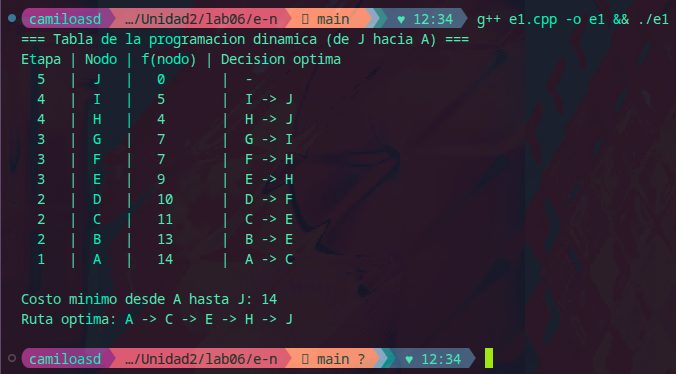
\includegraphics[width=0.8\textwidth]{../img/e1.png}
    \caption{Ejecución del ejercicio 1}
    \label{fig:e1}
\end{figure}

\subsection{Ejercicio 2}
Implementa \textbf{Fibonacci} de tres formas:
\begin{enumerate}
    \item Recursivo ingenuo
    \item Con memorización (top-down)
    \item Con tabulación (bottom-up)
\end{enumerate}
Compara sus tiempos de ejecución para $n = 10, 20$ y $30$.
\inputminted{cpp}{../e-n/e2.cpp}

\begin{itemize}
    \item Aquí se compara el cálculo de Fibonacci en tres formas: recursivo ingenuo, con memoización y con tabulación. El primero repite muchos subproblemas y es mucho más lento; la memoización evita repetir trabajo y la tabulación resuelve de abajo hacia arriba con el mejor rendimiento y menor costo computacional.
\end{itemize}

\begin{figure}[H]
    \centering
    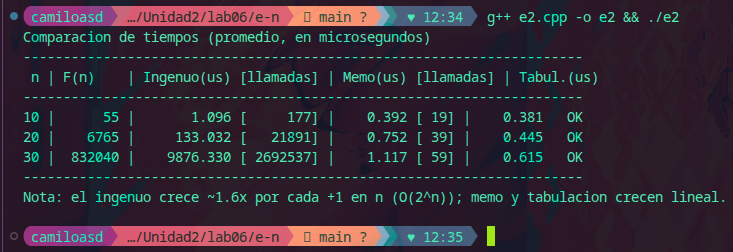
\includegraphics[width=0.8\textwidth]{../img/e2.png}
    \caption{Ejecución del ejercicio 2}
    \label{fig:e2}
\end{figure}

\subsection{Ejercicio 3}
Modifica el código del problema de la diligencia para que, cuando existan empates como el de D, se impriman \textbf{TODOS} los caminos óptimos encontrados, no solo uno.
\inputminted{cpp}{../e-n/e3.cpp}

\begin{itemize}
    \item En esta variante se modifica la lógica para conservar todos los caminos óptimos cuando hay empates. En lugar de guardar solo un sucesor, se guarda la lista de decisiones que alcanzan el mismo costo mínimo, y luego se recorren todas esas rutas con una búsqueda DFS para mostrar todos los caminos válidos.
\end{itemize}

\begin{figure}[H]
    \centering
    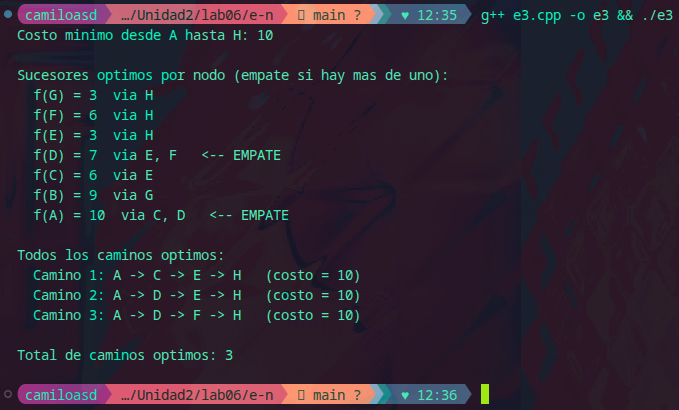
\includegraphics[width=0.8\textwidth]{../img/e3.png}
    \caption{Ejecución del ejercicio 3}
    \label{fig:e3}
\end{figure}

\subsection{Ejercicio 4}
Aplica la técnica \textbf{SRTBOT} para resolver un problema de camino de costo \textbf{MÁXIMO} (en vez de mínimo) sobre una malla de etapas similar a la del ejercicio resuelto.
\inputminted{cpp}{../e-n/e4.cpp}

\begin{itemize}
    \item Este ejercicio aplica la misma técnica de programación dinámica, pero buscando el máximo beneficio en lugar del mínimo costo. La estructura del algoritmo se mantiene: se resuelve de atrás hacia adelante con una recurrencia basada en el mejor valor futuro, y se guarda el camino o caminos de mayor ganancia.
\end{itemize}

\begin{figure}[H]
    \centering
    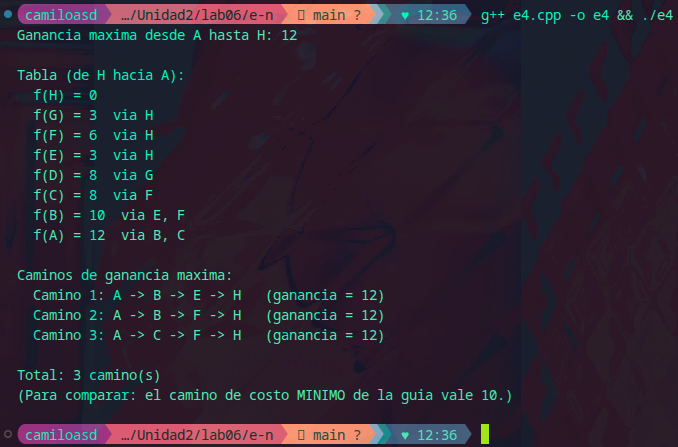
\includegraphics[width=0.8\textwidth]{../img/e4.png}
    \caption{Ejecución del ejercicio 4}
    \label{fig:e4}
\end{figure}

\subsection{Ejercicio 5}
Investiga y documenta un problema real (logística, finanzas, biología computacional) que pueda modelarse como un problema de decisión multietapa similar al de la diligencia, y explica cómo se definirían sus subproblemas.
\inputminted{cpp}{../e-n/e5.cpp}

\begin{itemize}
    \item En este caso se estudia un problema real de producción e inventario, donde cada mes debe decidir cuánto producir para satisfacer la demanda con el menor costo total. El estado incluye el mes y el inventario disponible, y la programación dinámica permite elegir la mejor producción considerando el costo de fabricar, almacenar y el futuro de cada periodo.
\end{itemize}

\begin{figure}[H]
    \centering
    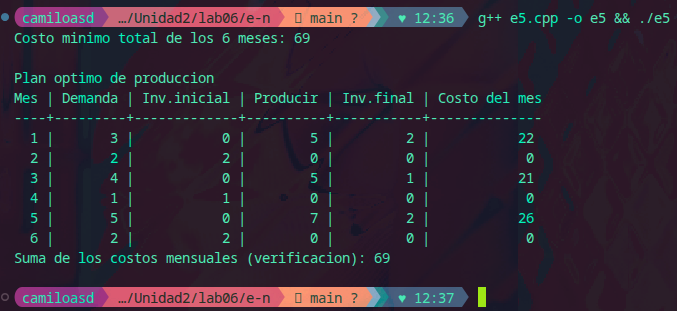
\includegraphics[width=0.8\textwidth]{../img/e5.png}
    \caption{Ejecución del ejercicio 5}
    \label{fig:e5}
\end{figure}

\section{Cuestionario}

\begin{enumerate}
    \item ¿Qué dos condiciones debe cumplir un problema para poder resolverse con Programación Dinámica? La respuesta es que debe presentar subproblemas superpuestos y una estructura óptima, es decir, la solución del problema completo debe poder construirse a partir de soluciones correctas de subproblemas más pequeños. Si el problema no repite trabajo ni puede descomponerse en decisiones donde cada parte contribuya a una solución global, entonces la técnica no aporta un beneficio real.
    \item ¿Cuál es la diferencia principal entre memorización y tabulación? La memorización es una estrategia top-down, que resuelve recursivamente y guarda los valores ya calculados para no repetirlos; en cambio, la tabulación sigue un enfoque bottom-up y llena la tabla desde los casos base hasta el estado final. Ambas son correctas, pero la manera de recorrer el problema y el uso de memoria son distintos.
    \item En la técnica SRTBOT, ¿qué garantiza específicamente el paso del orden topológico? El orden topológico garantiza que cada estado se calcule después de los estados de los que depende. Esto evita que una solución parcial use información aún no resuelta y permite que la ecuación de recurrencia tenga sentido al momento de evaluar un problema concreto.
    \item ¿Por qué el problema de la diligencia puede tener más de una solución óptima? Porque varias rutas distintas pueden llegar al mismo costo total, especialmente cuando existen empates entre decisiones alternativas. En esos casos, el algoritmo debe decidir si guarda solo una opción o conserva todas las que alcanzan el mismo valor óptimo, según el objetivo del problema.
    \item ¿Por qué aplicar Programación Dinámica a un algoritmo como Mergesort (Laboratorio 3) no traería ninguna mejora de eficiencia? Porque Mergesort ya divide el problema en subproblemas disjuntos y cada parte se resuelve solo una vez, sin superposición ni reutilización repetida de resultados. La programación dinámica se beneficia cuando un mismo subproblema aparece muchas veces, algo que no ocurre en la estrategia de divide y vencerás del ordenamiento.
\end{enumerate}

\section{Conclusiones}

La programación dinámica resultó ser una herramienta muy útil para comprender cómo un problema puede resolverse de manera inteligente sin explorar todo el espacio de soluciones. A lo largo del laboratorio se observó que la clave no está solo en encontrar una fórmula recursiva, sino en reconocer cuándo los subproblemas se repiten y cuándo la solución óptima de un estado puede construirse a partir de soluciones de estados anteriores. Esa idea fue la base para resolver la diligencia, Fibonacci, los caminos óptimos con empates y el problema de producción e inventario.

Una de las conclusiones más importantes es que la misma estructura conceptual se reutiliza en varios contextos: el problema de la diligencia, la optimización del camino máximo y la planificación de producción tienen la misma lógica general de estados, transiciones y costo acumulado. Lo que cambia es la interpretación del valor a optimizar y la forma en que se evalúan las decisiones. Esto muestra que la programación dinámica no es un algoritmo aislado, sino un enfoque de diseño general aplicable a una gran variedad de problemas de optimización.

También se evidenció la diferencia entre la recursión ingenua y las versiones más eficientes. En Fibonacci, la solución recursiva directa repite muchos cálculos y crece exponencialmente; la memoización reduce el trabajo guardando resultados ya calculados, mientras que la tabulación elimina la recursión y procesa los estados en orden lógico. Esto deja claro que, en muchos casos, el costo real no está solo en la formulación del problema, sino en cómo se organizan los cálculos y cómo se reutiliza la información.

Finalmente, el laboratorio permitió ver que la programación dinámica no solo sirve para encontrar una solución óptima, sino también para reconstruir el camino o la secuencia de decisiones que la alcanzan. Esto es especialmente relevante cuando hay empates o múltiples soluciones válidas, ya que la técnica puede guardar no solo el mejor valor, sino también todas las decisiones que lo sostienen. En ese sentido, la programación dinámica no es solo una estrategia de cálculo eficiente, sino también una forma de comprender la estructura interna del problema y de justificar matemáticamente por qué una solución es óptima.
\end{document}
